\chapter{Exercise 09}
\extitle{DataSpliter}
%******************************************************************************%
%                                                                              %
%                                 Interlude                                    %
%                         for Machine Learning module                          %
%                                                                              %
%******************************************************************************%

% ============================================== %
\section*{Interlude - Lost in Overfitting}
% ---------------------------------------------- %

The two previous exercises lead you, dear reader, to a very dangerous territory: the realm of \textbf{overfitting}.\\
You did not see it coming but now, you are in a bad situation...\\
\\
By increasing the polynomial degree of your model, you increased its \textbf{complexity}.  
Is it wrong?
Not always.
Some models are indeed very complex because the relationships they represent are very complex as well.\\
\\
But, if you look at the plots for the previous exercise's \textit{best model}, you should feel that something is wrong...\\
\\
% ============================================== %
\section*{Interlude - Something is rotten in the state of our model...}
% ---------------------------------------------- %
Take a look at the following plot. 

\begin{figure}[!h]
    \centering
    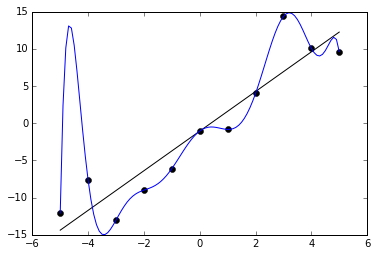
\includegraphics[scale=0.6]{assets/overfitt.png}
    \caption{Overfitting hypothesis}
\end{figure}

You can see that the prediction line fits each data point perfectly, but completely misses out on capturing the relationship between $x$ and $y$ properly.
And now, if we add some brand new data points to the dataset, we see that the predictions on those new examples are way off.

\begin{figure}[!h]
    \centering
    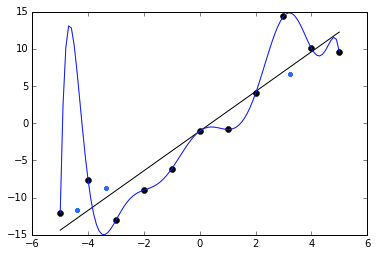
\includegraphics[scale=0.6]{assets/overfitt_with_dots.png}
    \caption{Generalization errors resulting from overfitting}
\end{figure}
This situation is called overfitting, because the model is doing an excessively good job at fitting the data.
It is literally bending over backward to account for the data's mini details.
But most of the data's irregularities are just noise, and they should in fact be ignored.
So because the model overfits, it can't generalize to new data.

% ============================================== %
\section*{Interlude - The training set, the test set, and the happy data scientist}
% ---------------------------------------------- %
To be able to detect overfitting, \textbf{you should always evaluate your model on new data}.\\
\\
New data means, data that your model hasn't seen during training.\\
\\
It's the only way to make sure your model isn't \textit{recalling}.
To do so, now and forever, you must always divide your dataset in (at least) two parts: one for the training, and one for the evaluation of your model.
\newpage
\turnindir{ex09}
\exnumber{09}
\exfiles{data\_spliter.py}
\exforbidden{sklearn}
\makeheaderfilesforbidden


% ================================= %
\section*{Objective}
% --------------------------------- %
Learn how to split a dataset into a \textbf{training set} and a \textbf{test set}.

% ================================= %
\section*{Instructions}
% --------------------------------- %
You must implement a function that \textbf{shuffles} and \textbf{splits} a dataset it into two parts: a \textbf{training set} and a \textbf{test set}.
\begin{itemize}
  \item Your function will shuffle and split the $X$ matrix while keeping a certain \textbf{proportion} of the examples for training, and the rest for testing.
  \item Your function will also shuffle and split the $y$ vector while making sure that the order of the rows in the output match the order of the rows in the split $X$ output.
\end{itemize}
In the \texttt{data\_spliter.py} file create the following function as per the instructions given below:\\
\\
\begin{minted}[bgcolor=darcula-back,formatcom=\color{lightgrey},fontsize=\scriptsize]{python}
def data_spliter(x, y, proportion):
    """Shuffles and splits the dataset (given by x and y) into a training and a test set,
      while respecting the given proportion of examples to be kept in the training set.
    Args:
      x: has to be an numpy.array, a matrix of dimension m * n.
      y: has to be an numpy.array, a vector of dimension m * 1.
      proportion: has to be a float, the proportion of the dataset that will be assigned to the
        training set.
    Return:
      (x_train, x_test, y_train, y_test) as a tuple of numpy.array
      None if x or y is an empty numpy.array.
      None if x and y do not share compatible dimensions.
      None if x, y or proportion is not of expected type.
    Raises:
      This function should not raise any Exception.
    """
    ... Your code ...
\end{minted}

\warn{
  \begin{itemize}
    \item The dataset has to be randomly shuffled \textit{before} it is split into training and test sets.
    \item Unless you use the same seed in your randomization algorithm, you won't get the same results twice.
  \end{itemize}
}

% ================================= %
\section*{Examples}
% --------------------------------- %
The following examples are just an indication of possible outputs. As long as you have shuffled datasets with their corresponding y values, your function is working correctly.\\
\\
\begin{minted}[bgcolor=darcula-back,formatcom=\color{lightgrey},fontsize=\scriptsize]{python}
import numpy as np
x1 = np.array([1, 42, 300, 10, 59]).reshape((-1, 1))
y = np.array([0, 1, 0, 1, 0]).reshape((-1, 1))

# Example 1:
data_spliter(x1, y, 0.8)
# Output:
(array([  1,  59,  42, 300]), array([10]), array([0, 0, 1, 0]), array([1]))

# Example 2:
data_spliter(x1, y, 0.5)
# Output:
(array([59, 10]), array([  1, 300,  42]), array([0, 1]), array([0, 0, 1]))

x2 = np.array([[  1, 42],
               [300, 10],
               [ 59,  1],
               [300, 59],
               [ 10, 42]])
y = np.array([0, 1, 0, 1, 0]).reshape((-1, 1))

# Example 3:
data_spliter(x2, y, 0.8)
# Output:
(array([[ 10,  42],
        [300,  59],
        [ 59,   1],
        [300,  10]]),
 array([[ 1, 42]]),
 array([0, 1, 0, 1]),
 array([0]))

# Example 4:
data_spliter(x2, y, 0.5)
# Output:
(array([[59,  1],
        [10, 42]]),
 array([[300,  10],
        [300,  59],
        [  1,  42]]),
 array([0, 0]),
 array([1, 1, 0]))
\end{minted}